\section{Практична частина}
\subsection{Схема дослідів з біполярним транзистором}
\begin{figure}[ht]
\centering
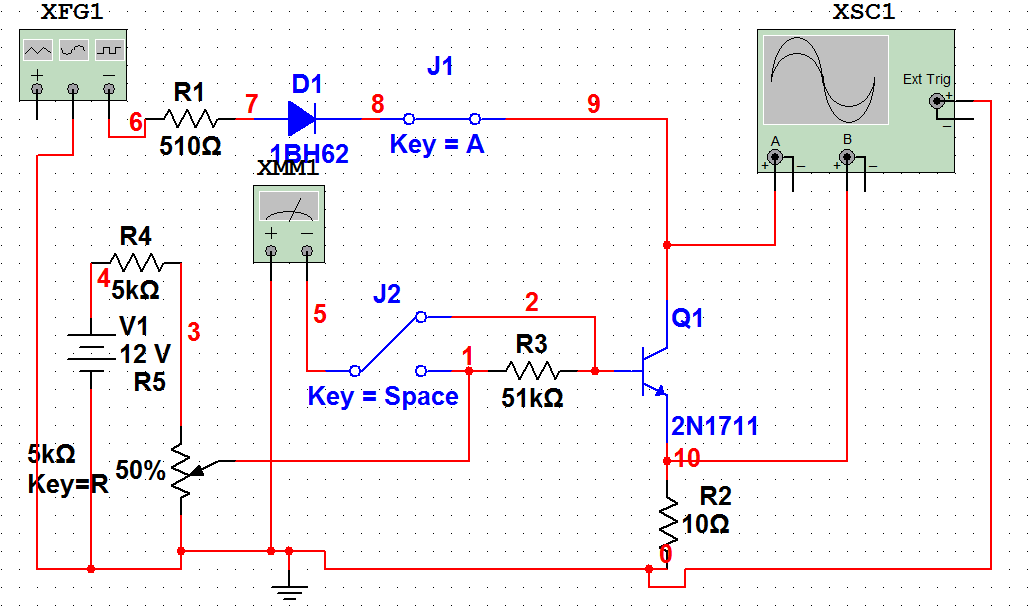
\includegraphics[width=1\linewidth]{Pic/first_1.png}
\end{figure}


\begin{figure}[ht]
\centering
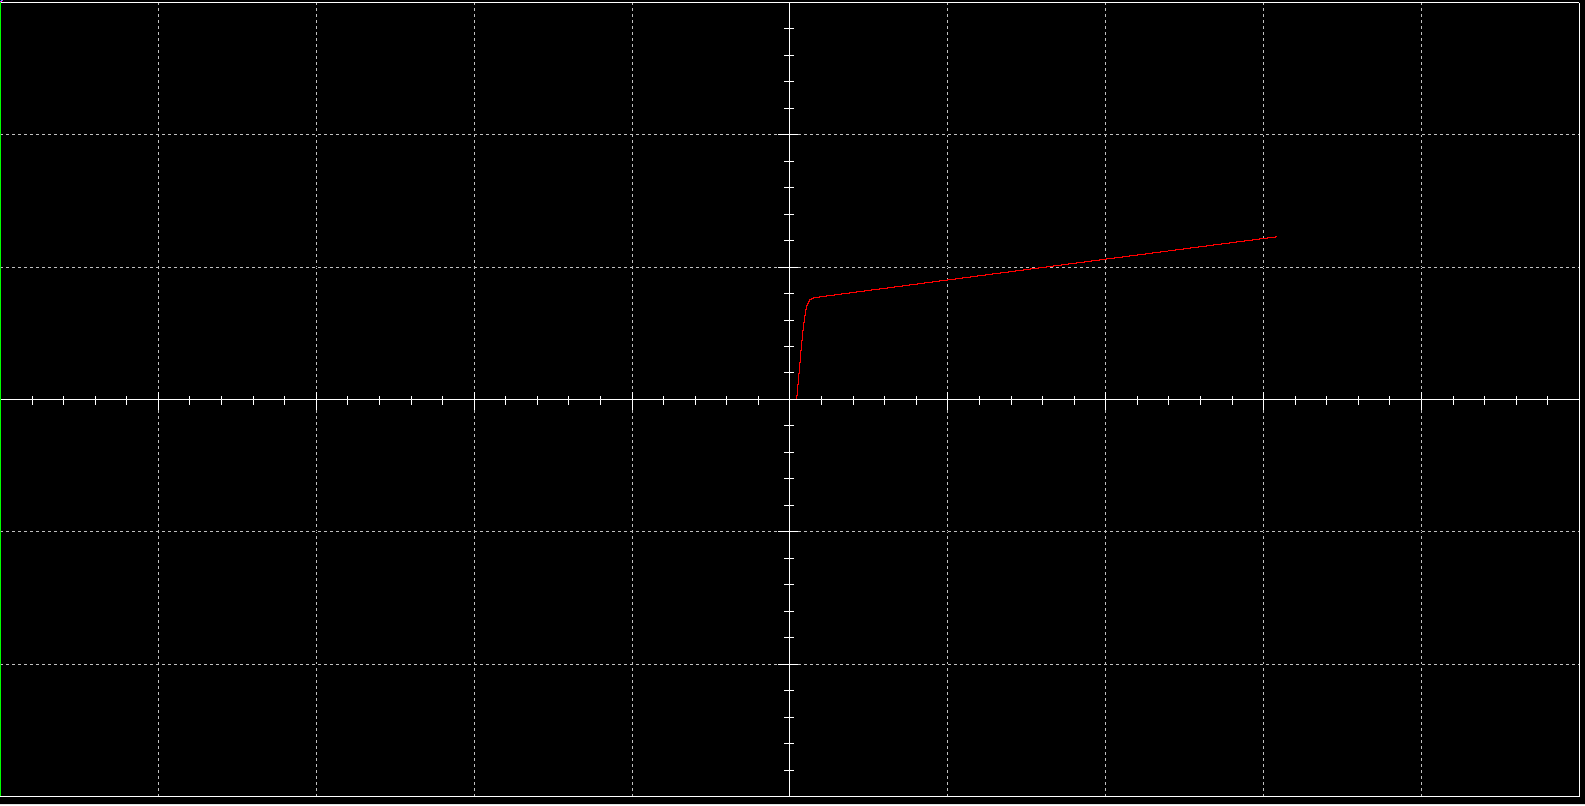
\includegraphics[width=1\linewidth]{Pic/first_2.png}
\end{figure}
\newpage


\subsection{Загальна схема дослідів з польовим транзистором}
\setlength{\parindent}{4em}


\begin{figure}[ht]
\centering
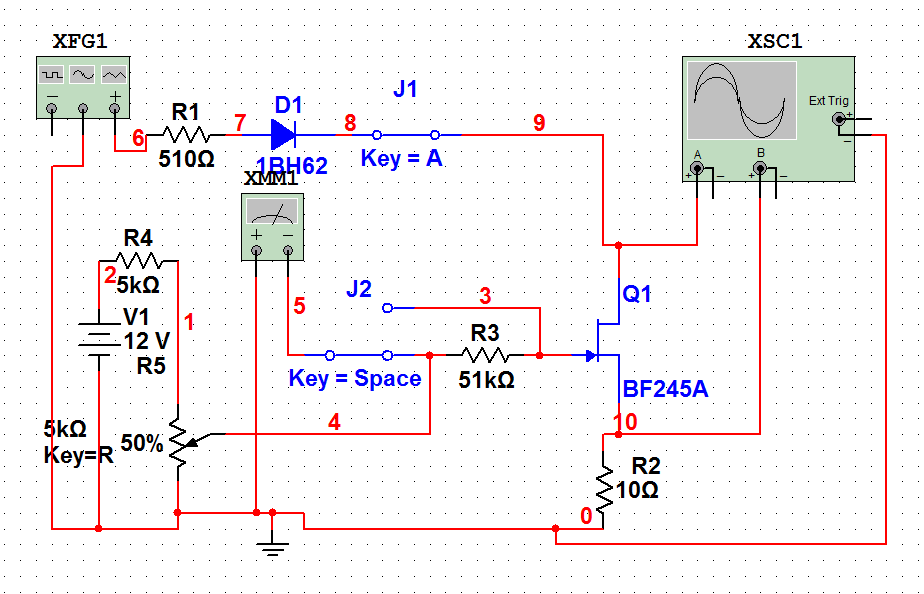
\includegraphics[width=1\linewidth]{Pic/shema.png}
\end{figure}
\newpage

\subsection{Покази приладів при 50$\%$}

\begin{figure}[ht]
\centering
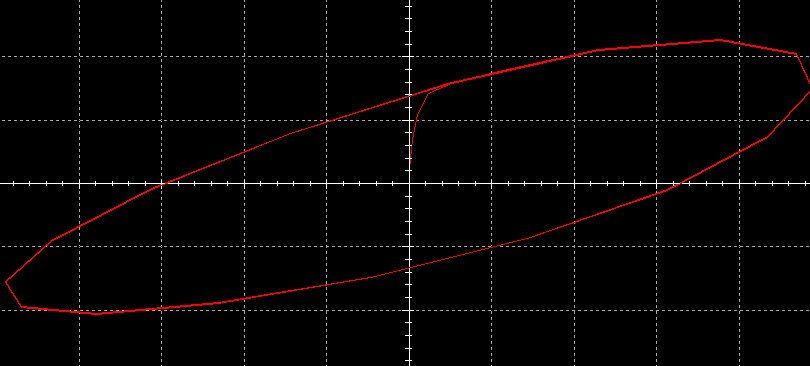
\includegraphics[width=1\linewidth]{Pic/51_1.png}
\end{figure}


\begin{figure}[ht]
\centering
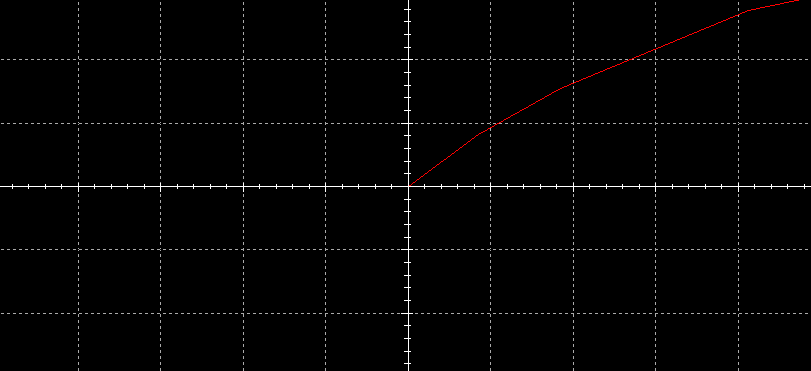
\includegraphics[width=1\linewidth]{Pic/51_2.png}
\end{figure}
\newpage

\subsection{Покази приладів при 30$\%$}

\begin{figure}[ht]
\centering
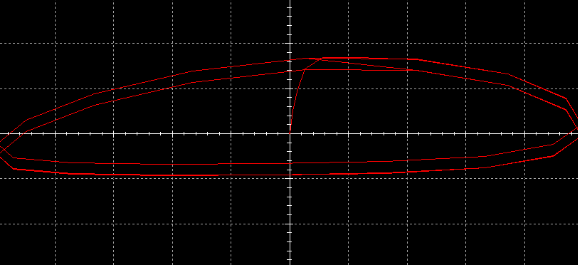
\includegraphics[width=1\linewidth]{Pic/30_1.png}
\end{figure}


\begin{figure}[ht]
\centering
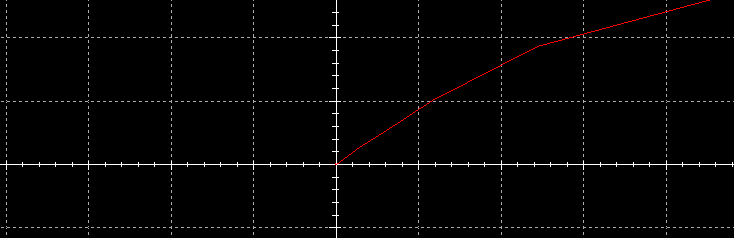
\includegraphics[width=1\linewidth]{Pic/30_2.png}
\end{figure}
\newpage

\subsection{Покази приладів при 90$\%$}

\begin{figure}[ht]
\centering
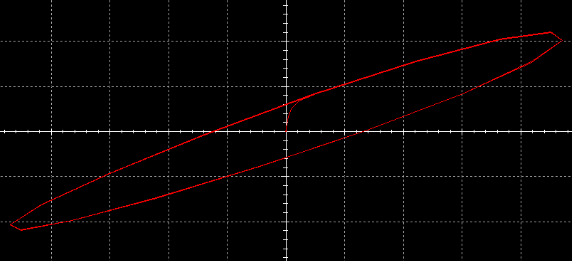
\includegraphics[width=1\linewidth]{Pic/90_1.png}
\end{figure}


\begin{figure}[ht]
\centering
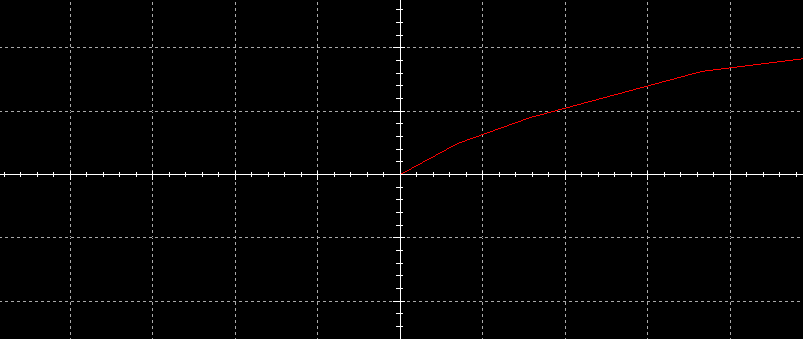
\includegraphics[width=1\linewidth]{Pic/90_2.png}
\end{figure}
\newpage
